\section{Coresets and Sensitivity Sampling}

In this work, we are using the method of coresets
(see for example~\cite{munteanu-coresets-introduction})
to approach the problem of data reduction for the probit model.
The idea behind coresets is, that when given a
dataset $\mathcal{D}$, we are interested in selecting
only a small subset of observations
$\mathcal{C} \subseteq \mathcal{D}$, such that the objective
function evaluated on the (possible reweighted) subset $\mathcal{C}$
does not differ too much
from the objective function evaluated on the original dataset $\mathcal{D}$.

This approach will allow us to estimate the model parameters
efficiently on the ideally much smaller set $\mathcal{C}$,
when a full optimization on $\mathcal{D}$ could already
be infeasible for big datasets.
We are thus following the paradigm of \textit{sketch-and-solve},
i.e. first reducing the size of the original dataset and then solving
the optimization problem on the reduced dataset.

In order to work out a formal definition of when we call a subset
$\mathcal{C} \subseteq \mathcal{D}$ a coreset in the context of
probit regression, we first have to slightly extend the
concept of the model matrix, as we will need it for the coreset
definition.

\begin{definition}[Scaled model matrix]
    Let $\mathcal{D}=\{(x_i, y_i)\}_{i=1}^n$ be a $d$-dimensional dataset.
    Let $z_i = (2y_i - 1)x_i$ for all i in $[n]$.
    Then we call the matrix $Z \in \mathbb{R}^{n \times d}$, where the
    $i$-th row consists of the vector $z_i$ for all $i \in [n]$,
    the scaled model matrix of $\mathcal{D}$.
\end{definition}

This definition of the scaled model matrix is nothing particularly new,
it just formalizes the concept of factoring the labels into the
model matrix, which we already encountered when dealing with the
parameter estimation in section~\ref{sec:parameter-estimation}.

We are now ready for the coreset definition:

\begin{definition}[Coreset]
    \label{def:coreset}
    Let $\mathcal{D}=\{(x_i, y_i)\}_{i=1}^n$ be a $d$-dimensional dataset
    with scaled model matrix $Z \in \mathbb{R}^{n \times d}$ and
    a vector of positive sample weights $w \in \mathbb{R}_{>0}^n$.
    Let $\mathcal{C} \subseteq \mathcal{D}$ be a subset of $\mathcal{D}$
    of size $|\mathcal{C}| = k$
    with scaled model matrix $C \in \mathbb{R}^{k \times d}$ and
    a vector of positive sample weights $u \in \mathbb{R}_{>0}^k$.
    Let $\frac{1}{2} > \epsilon > 0$.
    We call $\mathcal{C}$ a $(1+\epsilon)$-coreset of $\mathcal{D}$
    for probit regression, if
    \begin{equation*}
        (1-\epsilon)f_Z^w(\beta) \leq f_C^u(\beta) \leq (1+\epsilon)f_Z^w(\beta)
        \quad \forall \beta \in \mathbb{R}^d,
    \end{equation*}
    where $f_Z^w(\beta) = \sum_{i=1}^n w_i g(z_i^T \beta)$ is the
    weighted objective function of the probit model.
\end{definition}

The size parameter $k = |\mathcal{C}|$ of a coreset usually depends
on the desired approximation quality $\epsilon$, as well as on
specific problem characteristics, such as the number of observations
$n$ as well as the dimensionality $d$ of the dataset.
When constructing coresets, we are interested in keeping this parameter
low in comparison to the total size of the dataset, i.e. we
usually require that at least $k \in O(\log{n})$, so that
the data reduction is actually meaningful.

In the next section, we will investigate if there are any
guarantees that can be given regarding the coreset size
without imposing any further restrictions on the dataset.
We will find out, that in the general case, it can't
be guaranteed that a reasonably small coreset always exists.
As a consequence, we will later confine our research to a
specific class of datasets that we will call $\mu$-complex,
for which small upper bounds on the coreset size can be
derived.

\subsection{Do small coresets always exist?}

Before attempting to construct an algorithm that
is able to find small coresets, we first
have to investigate if such a goal is even attainable,
i.e. we have to make sure that small coresets even exist.

Without imposing any restrictions on the datasets, it turns out
that it is not difficult to find a counter example, i.e. to find
a dataset $\mathcal{D}$, such that no subset
$\mathcal{C} \subseteq \mathcal{D}$ of roughly logarithmic size
can be a coreset. This negative result has first been
proven in the context of logistic regression by the
authors of~\cite{on-coresets}, but it turns out that
the problematic dataset that admits no small coresets is
the same for probit regression as well.

This finding forces us to make a decision:
Do we have to give up our search for small coresets because
we now know that they don't always exist?
Or is there still hope, perhaps by imposing some (very reasonable)
restrictions on the class of datasets that we consider?
But before we can turn to this discussion, we first reproduce
the counter example for the general case with the following theorem.

\begin{theorem}
    \label{theorem:index}
    There exists a dataset $\mathcal{D}$ of size
    $|\mathcal{D}| = n$, such
    that any $(1+\epsilon)$-coreset $\mathcal{C}$ of $\mathcal{D}$
    for probit regression has a size $k = |\mathcal{C}|$
    of at least $k \in \Omega\left(\frac{n}{\log{n}}\right)$.
\end{theorem}
\begin{proof}
    We can construct such a  dataset by showing
    how coresets can be used in a
    communication protocol for the so called INDEX game,
    a communication game for two players, Alice and Bob, which
    works like this:

    Alice is given a random binary string $m \in \{0, 1\}^n$ of $n$ bits
    and Bob is given an index $i \in [n]$.
    The objective of the game is for Alice to send a message to Bob that allows
    Bob to obtain the value $m_i$ of Alice's binary string $m$.
    It was shown in~\cite{index}, that the minimum length of a message
    sent by Alice that still allows Bob to obtain $m_i$ with
    constant probability is in $\Omega(n)$ bits.
    We will now see, how a coreset for probit regression can be used
    to encode such a message.

    The first step is for Alice to convert her binary string $m$ into
    a dataset $\mathcal{D}$ as follows:
    For each entry $m_j$ of her binary string where $m_j = 1$, she adds
    a point
    \begin{equation*}
        x_j = \left( \cos{\left(2 \pi \frac{j}{n}\right)},
        \sin{\left(2 \pi \frac{j}{n}\right)}, 1 \right)^T
    \end{equation*}
    to her set $\mathcal{D}$ and labels it with $y_j = 1$,
    ending up with the dataset
    \begin{equation*}
        \mathcal{D} = \{(x_j, 1)\}_{j \in \{i \in [n]:\ m_i = 1 \}},
    \end{equation*}
    with all points being on the unit circle.

    The next step for her is to construct a
    $(1+\epsilon)$-coreset $\mathcal{C}$ of $\mathcal{D}$
    for probit regression with sample weights $u \in \mathbb{R}^k_{>0}$
    and to transmit both the coreset and the weight vector to Bob,
    which requires $O(\log(n))$ space for each point and
    weight.
    We will later see, how
    large the size $|\mathcal{C}|=k$ of this coreset must be,
    so that Bob can still
    obtain the value of $m_i$ with constant probability.

    As soon as Alice's coreset $\mathcal{C}$ arrives at Bob,
    Bob can use it to obtain the value of $m_i$.
    To do this, Bob first adds two new points
    \begin{equation*}
        q_1 = \left( \cos{\left(2 \pi \frac{i - 0.5}{n}\right)},
        \sin{\left(2 \pi \frac{i - 0.5}{n}\right)}, 1 \right)^T
    \end{equation*}
    and
    \begin{equation*}
        q_2 = \left( \cos{\left(2 \pi \frac{i + 0.5}{n}\right)},
        \sin{\left(2 \pi \frac{i + 0.5}{n}\right)}, 1 \right)^T
    \end{equation*}
    to the set and labels both points with $0$ (see figure~\ref{fig:index}),
    i.e. Bob now has the dataset
    \begin{equation*}
        \mathcal{C}' = \mathcal{C} \cup \{(q_1, 0)\} \cup \{(q_2, 0)\}.
    \end{equation*}

    Next, he uses this new dataset $\mathcal{C}'$ with
    scaled model matrix $C'$ to
    minimize the weighted objective function
    $f_{C'}^u$ of the probit model,
    by using the Newton-Raphson optimization algorithm.

    Taking a look at figure~\ref{fig:index}, it becomes evident,
    that Bobs points $q_1$ and $q_2$ are linearly separable from
    the other points if and only if Alice didn't add a point
    $x_i$, i.e. if $m_i = 0$.
    He can use the results of the optimization procedure to
    make a distinction between the two cases
    (which then allows him to determine the value of $m_i$)
    like this:

    In the case of $m_i=1$, Bobs points are not linearly separable from
    Alices original points, which means that there must occur at least one
    misclassification at a cost of $g(0) = \log(2)$ for the original
    loss function.
    Because Bobs dataset $\mathcal{C}'$ allows him to obtain a
    $(1 \pm \epsilon)$-approximation of the original cost function, he can
    check if the Newton-Raphson algorithm converges to
    a cost of at least $(1 - \epsilon) \log(2) \geq \frac{1}{2} \log(2)$
    for $\epsilon \leq \frac{1}{2}$.
    In this case, he knows that Alice must have added the point $x_i$,
    which means that $m_i=1$.

    Conversely, if at any point during the optimization procedure
    the cost function drops below
    $\frac{1}{2} \log(2)$
    and approaches zero, Bob knows that Alice didn't add the point
    $x_i$, because his dataset $\mathcal{C}'$ is linearly separable.
    This will allow him to conclude that $m_i = 0$.

    Let us now see, how large the size $k$ of Alice's coreset must be
    for this protocol to work with constant probability.
    In~\cite{index} it was shown, that the minimum length of a message
    that Alice must send in order for the protocol to work
    is in $\Omega(n)$ bits.
    Since each of the points that Alice created can be encoded in
    $\log(n)$ space, it follows from the lower bound that
    $\Omega(n) \subseteq \Omega(k \log(n))$, so $k$ must be in
    $\Omega\left(\frac{n}{\log(n)}\right)$.

    We can conclude, that if there existed a $(1 + \epsilon)$-coreset
    of $\mathcal{D}$
    for probit regression with size $k \in o\left(\frac{n}{\log(n)}\right)$,
    it would contradict the minimum message length of
    the INDEX communication game, which proves the theorem.
\end{proof}

\begin{figure}[h]
    \centering
    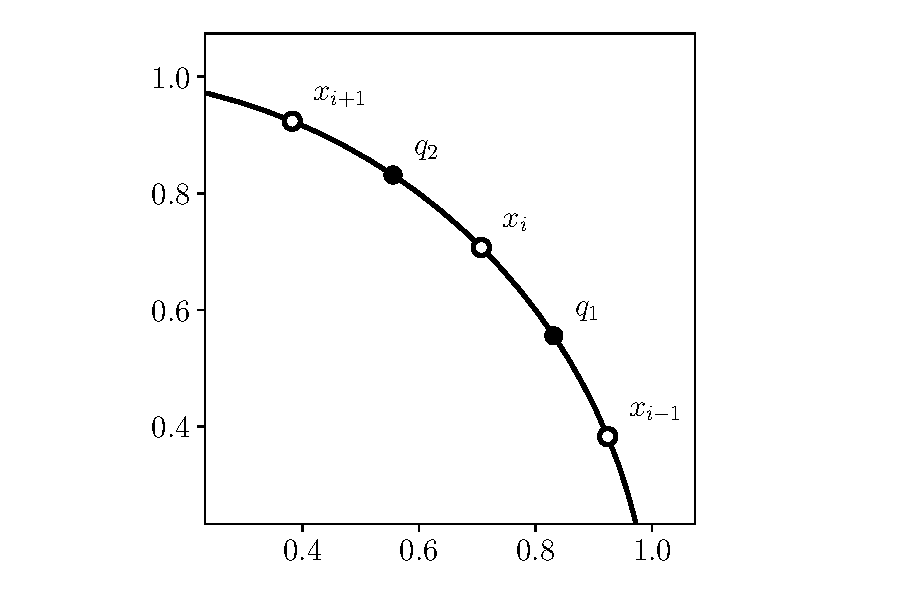
\includegraphics[width=0.8\textwidth]{figures/index.pdf}
    \caption{Bob places two points $q_1$ and $q_2$ in such a way
        on the unit circle, that they can be linearly seperated from the other
        points if and only if Alice didn't place a point at $x_i$.}
    \label{fig:index}
\end{figure}

We now have an example of a dataset for which no small coresets exist,
which implies that in the general case, without any restrictions,
there are no guarantees that it's even possible to find a small coreset.
But there is one thing that we have to note:
The counter example from the INDEX proof is by no means a
dataset that could ever be reasonably subjected to a probit analysis.
It consists of only positive labels! How can any inference ever
be possible in such a case? Further, it is easy to recognize,
that the counter example is linearly separable.
As we already saw in section~\ref{sec:parameter-estimation}, when
estimating the model parameters, the maximum likelihood estimate
only exists when the data is not linearly separable.
So yes, we found an example dataset for which no small coresets exist, but
does that mean that this particular "degenerate" example is relevant
to the attainment of our goal of constructing efficient data reduction
algorithms for the purpose of probit regression? Since the
maximum likelihood extimate doesn't even exist for this dataset,
it can be doubted, to say the least.

It therefore seems reasonable to impose some restrictions on the
datasets under study. Since we are exclusively dealing with
probit regression, it makes sense to restrict the
class of data sets to those, where a probit model can
at least be properly estimated, i.e. where the data is not linearly separable
and were the maximum likelihood estimate exists.

The authors of~\cite{on-coresets} were dealing with similar issues in
the context of logistic regression, so they decided to introduced a
measure, which they call $\mu$, that describes the degree of separability
of a dataset.
We are adapting this measure for probit regression in the following definition.

\begin{definition}($\mu$-complexity)
    \label{def:mu}
    Let $\mathcal{D}$ be a $d$-dimensional dataset of size
    $|\mathcal{D}|=n$ with scaled
    model matrix $Z \in \mathbb{R}^{n \times d}$, where
    $z_i \in \mathbb{R}^d$ constitutes the $i$-th
    row of $Z$ and let
    $w \in \mathbb{R}^n_{>0}$ be a vector of positive weights.
    Let $I_\beta^+ = \{i \in [n]:\ w_i z_i^T \beta > 0 \}$
    and let $I_\beta^- = \{i \in [n]:\ w_i z_i^T \beta < 0 \}$.
    Let
    \begin{equation*}
        \mu_w(\mathcal{D}) = \sup_{\beta \in \mathbb{R}^d \setminus \{0\}}
        \frac{\sum_{i \in I_\beta^+} w_i (z_i^T \beta)^2}
        {\sum_{i \in I_\beta^-} w_i (z_i^T \beta)^2}.
    \end{equation*}
    We call the dataset $\mathcal{D}$ with weight vector $w$
    $\mu$-complex, if there exists a $\mu \in \mathbb{R}$,
    such that $\mu_w(\mathcal{D}) \leq \mu$.
\end{definition}

The following lemma will be helpful later on:
\begin{lemma}
    \label{lemma:mu-inequalities}
    Let $\mathcal{D}$ be a $d$-dimensional and $\mu$-complex dataset of size
    $|\mathcal{D}|=n$ with scaled
    model matrix $Z \in \mathbb{R}^{n \times d}$ and weight
    vector $w \in \mathbb{R}^n_{>0}$ like in
    definition~\ref{def:mu}.
    The following relationship holds for all $\beta \in \mathbb{R}^d$:
    \begin{equation*}
        \mu^{-1} \sum_{i \in I_\beta^-} w_i (z_i^T \beta)^2
        \leq \sum_{i \in I_\beta^+} w_i (z_i^T \beta)^2
        \leq \mu \sum_{i \in I_\beta^-} w_i (z_i^T \beta)^2.
    \end{equation*}
\end{lemma}
\begin{proof}
    If $\mathcal{D}$ with weights $w$ is $\mu$-complex, then
    \begin{align*}
             & \frac{\sum_{i \in I_\beta^+} w_i (z_i^T \beta)^2}{\sum_{i \in I_\beta^-} w_i (z_i^T \beta)^2}
        \leq \mu_w(\mathcal{D}) \leq \mu                                                                     \\
        \iff &
        \sum_{i \in I_\beta^+} w_i (z_i^T \beta)^2
        \leq \mu \sum_{i \in I_\beta^-} w_i (z_i^T \beta)^2,
    \end{align*}
    which proves the second inequality.

    Considering that the labeling of a dataset is arbitrary, i.e. we
    could always switch the 1 labels for the 0 labels and vice versa
    (if we flip the sign of $\beta$
    accordingly),
    the following relationship is true as well:
    \begin{align*}
             & \frac{\sum_{i \in I_\beta^-} w_i (z_i^T \beta)^2}{\sum_{i \in I_\beta^+} w_i (z_i^T \beta)^2}
        \leq \mu_w(\mathcal{D}) \leq \mu                                                                     \\
        \iff &
        \sum_{i \in I_\beta^-} w_i (z_i^T \beta)^2
        \leq \mu \sum_{i \in I_\beta^+} w_i (z_i^T \beta)^2                                                  \\
        \iff &
        \mu^{-1} \sum_{i \in I_\beta^-} w_i (z_i^T \beta)^2
        \leq \sum_{i \in I_\beta^+} w_i (z_i^T \beta)^2,
    \end{align*}
    which proves the first inequality.
\end{proof}

There is a close relationship between $\mu$ and the linear
separability of a dataset as shown in the following theorem.

\begin{theorem}
    \label{theorem:mu-linear-separability}
    Let $\mathcal{D}$ be a $d$-dimensional dataset of size
    $|\mathcal{D}| = n$ like in definition~\ref{def:mu}
    and let $w \in \mathbb{R}^n_{>0}$ be a vector of
    positive weights.
    Then, the dataset
    $\mathcal{D}$ with weight vector $w$ is $\mu$-complex
    if and only if $\mathcal{D}$ is not linearly separable.
\end{theorem}
\begin{proof}
We first prove the "$\Rightarrow$" direction, i.e. we show
that if $\mathcal{D}$ is $\mu$-complex,
then it is not linearly separable.
We do this by proving the equivalent
contraposition that if $\mathcal{D}$ is linearly separable,
then it is not $\mu$-complex.

Let $S_0 = \{i \in [n]:\ y_i = 0\}$ and $S_1 = \{i \in [n]:\ y_i = 1\}$
like in definition~\ref{def:linear-separability}.
If $\mathcal{D}$ is linearly separable, then there exists
a $\beta \in \mathbb{R}^d \setminus \{0\}$, such that
\begingroup
\allowdisplaybreaks
\begin{align*}
                & \forall i \in S_0:\ x_i^T \beta \leq 0\quad \text{and}\quad \forall i \in S_1:\ x_i^T \beta \geq 0                       \\
    \iff        &                                                                                                                          \\
                & \forall i \in S_0:\ (-1) x_i^T \beta \geq 0\quad \text{and}\quad \forall i \in S_1:\ x_i^T \beta \geq 0                  \\
    \iff        &                                                                                                                          \\
                & \forall i \in S_0:\ (2y_i - 1) x_i^T \beta \geq 0\quad \text{and}\quad \forall i \in S_1:\ (2y_i - 1) x_i^T \beta \geq 0 \\
    \iff        &                                                                                                                          \\
                & \forall i \in S_0:\ z_i^T \beta \geq 0\quad \text{and}\quad \forall i \in S_1:\ z_i^T \beta \geq 0                       \\
    \iff        &                                                                                                                          \\
                & \forall i \in [n]:\ z_i^T\beta \geq 0                                                                                    \\
    \iff        &                                                                                                                          \\
                & I_\beta^- = \{ i \in [n]:\ w_iz_i^T\beta < 0\} = \emptyset                                                               \\
    \iff        &                                                                                                                          \\
                & \sum_{i \in I_\beta^-} w_i (z_i^T \beta)^2 = 0                                                                           \\
    \Rightarrow &                                                                                                                          \\
                & \mu_w(\mathcal{D}) \geq \frac{\sum_{i \in I_\beta^+} w_i (z_i^T \beta)^2}
    {\sum_{i \in I_\beta^-} w_i (z_i^T \beta)^2} = \infty,
\end{align*}
\endgroup
which means that $\mathcal{D}$ is not $\mu$-complex.

It now remains to prove the "$\Leftarrow$" direction, i.e. to
show that if $\mathcal{D}$ is not linearly separable,
then it is $\mu$-complex. Again, we do this by proving the
equivalent contraposition that if $\mathcal{D}$ is not
$\mu$-complex, then it is linearly separable.

The first step in order to do so is to show that we can restrict the
supremum in $\mu_w(\mathcal{D})$ to finite $\beta$ with
$\lVert \beta \rVert = 1$:
\begin{align*}
    \mu_w(\mathcal{D}) & = \sup_{\beta \in \mathbb{R}^d \setminus \{0\}}
    \frac{\sum_{i \in I_\beta^+} w_i (z_i^T \beta)^2}
    {\sum_{i \in I_\beta^-} w_i (z_i^T \beta)^2}                                         \\ & =
    \sup_{\beta \in \mathbb{R}^d \setminus \{0\}}
    \frac{\sum_{i \in I_\beta^+} \frac{1}{\lVert \beta \rVert^2}w_i (z_i^T \beta)^2}
    {\sum_{i \in I_\beta^-} \frac{1}{\lVert \beta \rVert^2} w_i (z_i^T \beta)^2}         \\
                       & =
    \sup_{\beta \in \mathbb{R}^d \setminus \{0\}}
    \frac{\sum_{i \in I_\beta^+} w_i \left(z_i^T \frac{\beta}{\lVert \beta \rVert}\right)^2}
    {\sum_{i \in I_\beta^-}  w_i \left(z_i^T \frac{\beta}{\lVert \beta \rVert}\right)^2} \\
                       & =
    \sup_{\tilde\beta \in \mathbb{R}^d,\ \lVert \tilde\beta \rVert = 1}
    \frac{\sum_{i \in I_\beta^+} w_i \left(z_i^T \tilde\beta \right)^2}
    {\sum_{i \in I_\beta^-}  w_i \left(z_i^T \tilde\beta \right)^2},
\end{align*}
which lets us conclude that even in the supremum, both expressions
$\sum_{i \in I_\beta^+} w_i (z_i^T \beta )^2$
and
$\sum_{i \in I_\beta^-}  w_i (z_i^T \beta )^2$
are finite.
This means that if $\mathcal{D}$ is not $\mu$-complex, then
the denominator must be zero, i.e. it must hold that there exists
a $\beta \in \mathbb{R}^d \setminus \{0\}$ such that
\begin{equation*}
    \sum_{i \in I_\beta^-}  w_i (z_i^T \beta )^2 = 0.
\end{equation*}

From here, we can follow the same chain of equivalences that we
showed when proving the "$\Rightarrow$"-direction of the theorem,
which leads us directly to the fact, that $\mathcal{D}$ in this case must
be linearly separable, which concludes the proof.
\end{proof}

As we already noted in section~\ref{sec:parameter-estimation},
linear separability is also closely related to the existence
of the maximum likelihood estimate in the probit model.
The next theorem uses the relationship between $\mu$ and
linear separability to show the connection between $\mu$
and the existence of the maximum likelihood estimate.

\begin{theorem}
    Let $\mathcal{D}$ be a $d$-dimensional dataset.
    Then, the maximum likelihood estimate $\tilde\beta$ for the probit
    model exists if and only if $\mathcal{D}$ is $\mu$-complex.
\end{theorem}
\begin{proof}
    This is a direct corollary from theorem~\ref{theorem:probit-existence}
    and theorem~\ref{theorem:mu-linear-separability}.
\end{proof}

In the following parts of this work, we will derive efficient upper
bounds on the coreset size for $\mu$-complex datasets.
In order to do this, we first introduce a theoretic
framework that we use for the coreset construction which
is based on the concept of sensitivities.

\subsection{The Sensitivity Framework}

After having imposed some reasonable restrictions on the
datasets under study, it is now time to think about
how an algorithm that selects a coreset
$\mathcal{C} \subseteq \mathcal{D}$ could be constructed.
One of the first ideas that come to mind to solve such a problem
is the process of uniform random sampling.
After all, why don't we just randomly select a subset of
points from $\mathcal{D}$ of the desired size, where
each datapoint is assigned an equal probability of
being selected?
Wouldn't that already solve our problem?

The issue with this approach is that it cannot be guaranteed
that such a uniform random sample will yield a coreset,
i.e. a subset of $\mathcal{D}$ that helps us to obtain a
$(1 \pm \epsilon)$-approximation of the original loss function.
As we will later see in the experiments section, uniform sampling
works reasonably well when the data is well behaved, but fails
terribly when there are a few very important datapoints that
it tends to miss.
Intuitively speaking,
if there are lots of points in a dataset that don't influence the
loss function much, but only a few points that have a big impact
on the loss function, uniform sampling fails because it tends
to miss the few very important points.

It turns out, that one way to remedy the downsides of uniform sampling
is to include a measure of importance in the sampling distribution.
Instead of sampling each datapoint with equal probability,
why don't we construct our sampling distribution in such a way,
that the impact of each point on the loss function is taken into
account? This way, more important points would be assigned
a higher probability of being sampled and less important points
would conversely be assigned a lower sampling probability.
This idea forms the basis of the so called
\textit{sensitivity framework}, an algorithmic framework
introduced in~\cite{feldman-langberg-coresets}
(see also \cite{big-data-tiny-data}), that aims to
find coresets by randomly sampling points proportional to
their importance for the loss function.

In the sensitivity framework, the importance of a point
in a dataset can be thought of the maximum proportion of
the loss function that it can take up in the worst case.
To formalize this intuition, the sensitivity framework shifts
the representation of a dataset as a collection of
points towards the representation as a collection of
\textit{functions}, where each function represents the
loss of a point.
To explain what that means, consider the dataset
$\mathcal{D} = \{(x_i, y_i)\}_{i=1}^n$ with scaled model
matrix $Z$, i.e. the rows of $Z$ are given by the vectors
$z_i = -(2y_i-1)x_i$ and the loss function is given by
$f(\beta) = \sum_{i=1}^n w_ig(z_i^T\beta)$, where
$w_1, ..., w_n$ are positive weights.
From now on, we will assign to each point in the dataset the
function $g_i(\beta) = g(z_i^T\beta)$, that represents its
individual contribution to the overall loss function.
This way, we can equivalently represent the dataset $\mathcal{D}$
as the set of functions $F = \{g_1, ..., g_n\}$.

Having made this conceptual change of representing a dataset as
a set of functions, we can now use this new representation to
formalize the concept of importance for each point, according
to wich we later want to sample.
As already hinted at, the importance of a point will be the
maximum fraction of the loss function, that the loss of the specific
point will take up in the worst case.
This worst case importance is also called the \textit{sensitivity}
of a point, and it was first introduced in
\cite{langberg-schulman-sensitivities}.
A formal definition of this concept, which forms
the basis of the sensitivity framework, is given below.

\begin{definition}[\cite{langberg-schulman-sensitivities}]
    \label{def:sensitivity}
    Let $F = \{ g_1, ..., g_n \}$ be a set of functions,
    $g_i: \mathbb{R}^d \rightarrow \mathbb{R}_{\geq 0}, \ i \in [n]$
    and let $w \in \mathbb{R}^n_{>0}$ be a vector of positive weights.
    The sensitivity of $g_i$ for $f_w(\beta) = \sum_{i=1}^n w_i g_i(\beta)$ is defined as
    \begin{equation*}
        \varsigma_i = \sup_{\beta \in \mathbb{R}^d, \ f_w(\beta) > 0} \frac{w_i g_i(\beta)}{f_w(\beta)}.
    \end{equation*}
    The total sensitivity, i.e. the sum of the sensitivities is $\mathfrak{S} = \sum_{i=1}^n \varsigma_i$.
\end{definition}

The idea behind the sensitivity framework is to sample from a
distribution, where the sampling probabilities are determined by
the sensitivities, i.e. the worst case importance of each point
in the dataset.
But there is one issue remaining: The true sensitivities
$\varsigma_1, ..., \varsigma_n$ are unknown, and as
pointed out in~\cite{braverman-feldman-coresets}, their
computation requires solving the original optimization problem,
which we wanted to avoid in the first place.
Luckily, there exists a simple workaround:
Instead of sampling proportionally to the true sensitivities,
we can instead also sample proportionally to
upper bounds $s_i$, where $s_i \geq \varsigma_i$, that are
potentially easier to compute.

There is one caveat though, that we have to take into account:
We will later see, that in the sensitivity framework, the
size of the coreset that we obtain through sampling proportionally
to upper bounds of the sensitivities, is directly influenced
by the sum of said bounds: $S = \sum_{i=1}^n s_i$.
It follows, that we have to find bounds that are as tight as
possible, so that our coreset won't be unnecessarily large.

The way in wich the authors of~\cite{feldman-langberg-coresets}
were able to show, that sampling proportionally to upper bounds of the
sensitivities can lead to provably small coresets,
was to relate the concept of sensitivities to
the theory of so-called \textit{range spaces} and
the \textit{VC-dimension}
(see for example \cite{computational-learning-theory} for an
introduction to the VC-dimension).
We introduce these concepts in the following definitions, because
they will also turn out to be of crucial importance to the
size of our coresets.

\begin{definition}[\cite{feldman-langberg-coresets}]
    \label{def:range-space}
    A range space is a pair $\mathfrak{R} = (F, \textup{ranges})$, where F is a set
    and $\textup{ranges}$ is a family (set) of subsets of F.
\end{definition}

\begin{definition}[\cite{feldman-langberg-coresets}]
    \label{def:vc-dimension}
    The VC-dimension $\Delta(\mathfrak{R})$ of a range space
    $\mathfrak{R} = (F, \textup{ranges})$ is
    the size $|G|$ of the largest subset $G \subseteq F$ such that
    \begin{equation*}
        \left| \left\{ G \cap R \ | \ R \in \textup{ranges} \right\} \right|
        = 2^{|G|},
    \end{equation*}
    i.e. $G$ is shattered by $\textup{ranges}$.
\end{definition}

The most important part to understand about the two preceding definitions
is the concept of \textit{shattering}.
Given a set $F$, a set of subsets of $F$ called ranges and a subset
$G \subseteq F$, what does it mean if $G$ is shattered by ranges?
Definition~\ref{def:vc-dimension} says, that the set of intersections
between $G$ and ranges must be equal to $2^{|G|}$, which is exactly
the size of the set of all subsets of $G$.
It follows, that for $G$ to be shattered by ranges, every subset
of $G$ must be a subset of at least one of the sets in ranges,
that isn't already occupied by another subset of $G$.
From this it also immediately follows, that if $G$ is shattered by
ranges, then every subset of $G$ is also shattered by ranges.
Thus, the VC-dimension of the range space that is given by $F$ and
ranges is simply the size of the largest subset $G \subseteq F$,
such that every subset of
$G$ appears in at least one element of ranges, where each such element
can account for at most one subset of $G$.

Instead of dealing with arbitrary sets like in
Definition~\ref{def:range-space} and Definition~\ref{def:vc-dimension},
we are specifically dealing with a set of functions
$F = \{g_1, ..., g_n\}$, that represents our dataset.
In the next definition, we will see, how such a set of functions
can be used to \textit{induce} a range space, which will
be of crucial importance when limiting the size of
our coresets later on.

\begin{definition}[\cite{feldman-langberg-coresets}]
    \label{def:induced-range-space}
    Let $F$ be a finite set of functions mapping from $\mathbb{R}^d$ to
    $\mathbb{R}_{\geq 0}$.
    For every $\beta \in \mathbb{R}^d$ and $r \geq 0$, let
    \begin{equation*}
        \textup{range}(F, \beta, r) = \left\{ f \in F \ | \  f(\beta) \geq r  \right\}
    \end{equation*}
    and let
    \begin{equation*}
        \textup{ranges}(F) = \left\{ \textup{range}(F, \beta, r) \ | \ \beta \in \mathbb{R}^d, \ r \geq 0  \right\}.
    \end{equation*}
    Then we call $\mathfrak{R}_F := (F, \textup{ranges}(F))$ the range space induced by F.
\end{definition}

To understand what it means for a set of functions $F$ to induce
a range space, consider that we can always partition the set
of functions into two disjoint subsets by choosing
a specific $\beta$ and applying a threshold $r$:
Every element in $F$ with a value of $f(\beta) \geq r$ goes to
one subset, the remainder goes to the other subset.
Considering that our functions actually represent datapoints,
each value of $\beta$ and $r$ give one way to partition the
datapoints into two disjoint subsets.
Thus, the set $\text{ranges}(F)$ in Definition~\ref{def:induced-range-space}
can be thought of the set of all possible partitions of
functions (datapoints), that can be obtained for all
possible $\beta \in \mathbb{R}^d$ and $r \geq 0$ and the
VC-dimension of the induced range space is the size of the
largest set of datapoints, that can be arbitrarily partitioned
by different values of $\beta$ and $r$.

We are now ready for the full theorem that relates sensitivity sampling
to the theory of range spaces and the VC-dimension, which forms
the core of the sensitivity framework.
Its original version goes back to~\cite{feldman-langberg-coresets}
and it was further improved in~\cite{braverman-feldman-coresets}.
The version we are presenting here is a slightly
adapted variant introduced in~\cite{big-data-tiny-data}:

\begin{theorem}[\cite{big-data-tiny-data}]
    \label{theorem:sensitivity-framework}
    Let $F = \{ g_1, ..., g_n \}$ be a finite set of functions
    mapping from $\mathbb{R}^d$ to $\mathbb{R}_{\geq 0}$.
    Let $w \in \mathbb{R}^n_{>0}$ be a vector of positive weights.
    Let $\epsilon, \delta \in (0, \frac{1}{2})$.
    Let $s_i \geq \varsigma_i$ be upper bounds of the sensitivities and
    let $S = \sum_{i=1}^n s_i$.
    Given $s_i$, one can compute in time $O(|F|)$ a set
    $R \subseteq F$ of
    \begin{equation*}
        |R| \in O \left( \frac{S}{\epsilon^2} \left( \Delta \log S + \log \left( \frac{1}{\delta} \right) \right) \right)
    \end{equation*}
    weighted functions, such that with probability $1 - \delta$ we have
    for all $\beta \in \mathbb{R}^d$ simultaneously
    \begin{equation*}
        (1-\epsilon) \sum_{g_i \in F} w_i g_i(\beta) \leq \sum_{g_j \in R} u_j g_j(\beta) \leq (1 + \epsilon) \sum_{g_i \in F} w_i g_i(\beta).
    \end{equation*}
    Each element of $R$ is sampled independently with probability
    $p_i = \frac{s_i}{S}$ from $F$, $u_j = \frac{S w_i}{s_i |R|}$
    denotes the weight of a function $g_j \in R$ that corresponds to
    $g_i \in F$ and $\Delta$ is an upper bound on the
    VC-dimension of the range space $\mathfrak{R}_{F^\ast}$ induced by
    $F^\ast$, where $F^\ast$ is the set of functions $g_i \in F$
    scaled by $\frac{S w_i}{s_i |R|}$, i.e.
    $F^\ast = \left\{ \frac{S w_i}{s_i |R|} g_i(\beta) \ |\ i \in [n] \right\}$.
\end{theorem}

The set of functions $R \subseteq F$ with weights $u$ is of course
a representation of
the coreset that we are interested in.
As Theorem~\ref{theorem:sensitivity-framework} tells us, the
size of this coreset depends on both, the sum of the sensitivity bounds
as well as the VC-dimension of the range space induced by $F^\ast$,
a reweighted version of $F$.

Another thing to note is that Theorem~\ref{theorem:sensitivity-framework}
introduces a failure probability $\delta$, which also influences the
size of the coreset. The reason why we need this new parameter becomes
clear when considering, that the coreset is selected by random sampling,
i.e. the coreset-construction process is probabilistic and
probabilistic processes can fail. This failure probability is reflected
by the parameter $\delta$.

Equipped with Theorem~\ref{theorem:sensitivity-framework}, we now have
a clear roadmap to follow in the pursuit of our goal of finding a
coreset construction
algorithm. We know, that we have to find small upper bounds on
the sensitivities of our function set $F = \{g_1, ..., g_n\}$
for the purpose of random sampling and at the
same time, we also know that we have to control the VC-dimension of the
range space of $F^\ast$.
Thus, bounding the sensitivities as well as bounding the VC-dimension
are the main challenges of the next section.


\subsection{Constructing the Coreset}

Without any point of reference, the task of finding tight
and efficiently computable upper bounds
on the sensitivities seems rather challenging.
How are we supposed to find those ominous bounds and on top of that,
how can we make sure that their sum will be small?
It helps to remind ourselves of the original problem that the sensitivities
were designed to solve. Instead of sampling every point with equal
probability, the sensitvities were introduced to include the importance
of each point into the sampling process.
But what if similar importance distributions already existed?
Could it be possible to choose an existing importance distribution
and relate it to the concept of sensitivities in order to
obtain upper bounds?

It turns out, that there is one importance sampling
distribution that is particularly helpful in the context of our problem:
The so-called statistical leverage scores (see for example
\cite{leverage-scores-drineas}).
For a dataset $\mathcal{D} = \{(x_i, y_i)\}_{i=1}^n$ with model
matrix $X$, the statistical leverage score of the $i$-th observation is
given by $\ell_i = x_i^T(X^TX)^{-1}x_i$.
Intuitively speaking, $\ell_i$ is a measure of the uniqueness of a given
observation $x_i$. If there aren't many
data points close to $x_i$, i.e. we can consider $x_i$ to be
unique, then the leverage score of $x_i$
is high. On the other hand, if there are a lot of other data points
close to $x_i$, i.e. $x_i$ is not unique, then the leverage score
is low. When using leverage scores as a sampling distribution, we
give a higher weight to points that are unique and different from
the other points, compared to points that are surrounded by a lot
of similar other points.

To better understand what that means, a visualization of the statistical
leverage scores of an artificially generated two dimensional dataset
is given in figure~\ref{fig:leverage-scores} as an example.
We can see, that most of the datapoints that are crowding the
center of the dataset have rather low leverage scores, but the further
out the points are located relatively to the center, the higher
the leverage scores become.
Particularly, there is a small group of outliers in the
top right of the coordinate system, and we can see that their leverage
scores are almost four times as high as the leverage scores
of the points in the center. Thus, when sampling points proportionally
to their leverage scores, we are less likely to miss outliers in
the data that could potentially have a high impact on the loss function.

\begin{figure}[ht!]
    \centering
    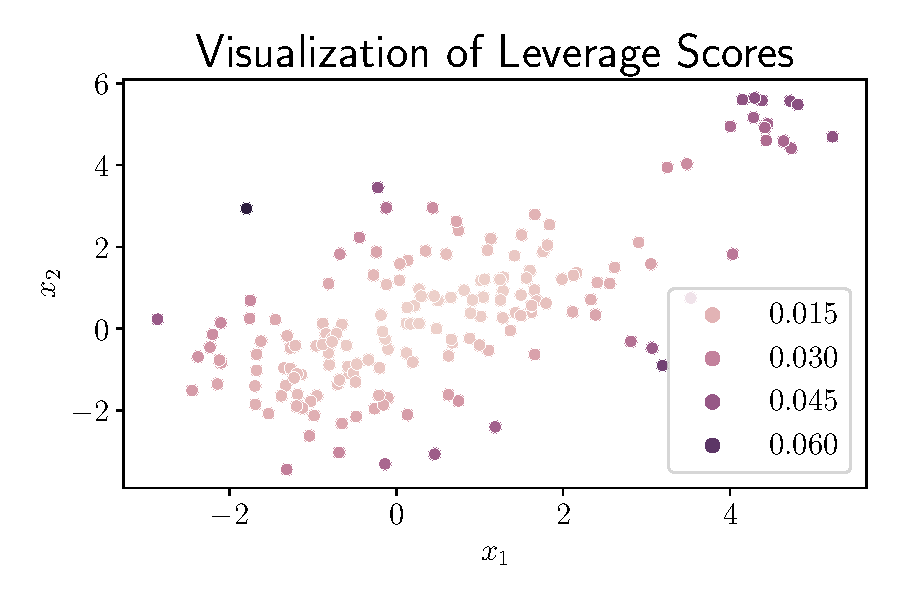
\includegraphics[width=.7\linewidth]{figures/leverage_scores_visualization.pdf}
    \caption{Visualization of the statistical leverage scores of an
        artificial two dimensional dataset. Darker colors indicate a higher
        leverage score than lighter colors.}
    \label{fig:leverage-scores}
\end{figure}

An alternative way of defining the leverage scores, which will
be particularly important to us when mathematically deriving
the sensitivity bounds later on, is to specify them as
the squared row norms of an orthonormal basis of the model matrix
$X \in \mathbb{R}^{n \times d}$.
Such an orthonormal basis can for example be obtained
by computing a so-called $QR$-decomposition of $X$
(see for example \cite{matrix-computations}), where
$X = QR$ is factorized into an orthonormal matrix
$Q \in \mathbb{R}^{n \times d}$ and an upper triangular
matrix $R \in \mathbb{R}^{d \times d}$.

Our goal in this section is to adapt the leverage scores in
such a way, that we can obtain tight upper bounds on the sensitivities.
But we are not quite ready for that yet.
Before we can get there, we first have to focus our attention back
to the probit loss function $g(x)$, because it turns out that in order
to bound the sensitivities by using the leverage scores, we first
have to cover some important properties of $g(x)$.

\subsubsection{A closer examination of the probit loss}

In order to find bounds on the sensitivities, we also
need bounds on the probit loss
$g(x) = \ln\left( \frac{1}{1 - \Phi(x)} \right)$.
The first bound that we will derive holds for all $x \geq 0$
and shows that $g(x)$ grows at least like a quadratic function.
Next, we will show that for all $x \geq 2$, $g(x)$ is upper
bounded by a quadratic function, and thus $g(x)$ asymptotically
grows like a quadratic function.
Both of these bounds will turn out to be helpful later
on. They are proven in lemma \ref{lemma:lower-bound}
and lemma \ref{lemma:upper-bound}.

\begin{lemma}
    \label{lemma:lower-bound}
    Let $g(x) = \ln \left( \frac{1}{1 - \Phi(x)}\right)$.
    Then, for all $x \geq 0$, it holds that:
    \begin{equation*}
        \frac{1}{2} x^2 \leq g(x).
    \end{equation*}
\end{lemma}
\begin{proof}
    We first show the claim for all $x \geq 1$, by using the following
    inequality:
    \begin{align*}
        \Phi(-x) & = \frac{1}{\sqrt{2 \pi}} \int_{-\infty}^{-x} \exp{ \left(-\frac{1}{2} t^2 \right)} dt       \\
                 & \leq \frac{1}{\sqrt{2 \pi}} \int_{-\infty}^{-x} -t \exp{ \left(-\frac{1}{2} t^2 \right)} dt \\
                 & = \frac{1}{\sqrt{2 \pi}} \exp{\left( -\frac{1}{2} x^2 \right)}                              \\
                 & \leq \exp{\left( -\frac{1}{2} x^2 \right)}.                                                 \\
    \end{align*}
    In the next step, we use this inequality to show that for $x \geq 1$:
    \begin{gather*}
        e^{g(x)} = e^{\ln \left( \frac{1}{1 - \Phi(x)} \right)} = \frac{1}{\Phi(-x)} \geq e^{\frac{1}{2} x^2}\\
        \iff \\
        g(x) \geq \frac{1}{2} x^2,
    \end{gather*}
    which proves the bound for $x \geq 1$.

    Let us now turn to the case when $0 \leq x \leq 1$.
    Both $g(x)$ and $\frac{1}{2}x^2$ are monotonically increasing
    and continuous functions for $0 \leq x \leq 1$.
    Making use of the fact that $g(0) > \frac{1}{2}$, it follows
    for all $0 \leq x \leq 1$, that
    \begin{equation*}
        g(x) \geq g(0) > \frac{1}{2} = \max_{0 \leq x \leq 1} \frac{1}{2} x^2 \geq \frac{1}{2} x^2,
    \end{equation*}
    which concludes the proof.
\end{proof}

\begin{lemma}
    \label{lemma:upper-bound}
    Let $g(x) = \ln \left(\frac{1}{1 - \Phi(x)}\right)$.
    Then, for all $x \geq 2$, it holds that:
    \begin{equation*}
        g(x) \leq x^2.
    \end{equation*}
\end{lemma}
\begin{proof}
    In~\cite{gaussian_bounds}, it was shown that the following inequality
    holds for all $x \geq 0$:
    \begin{equation*}
        \Phi(-x) \geq \frac{1}{\sqrt{2 \pi}} \frac{x}{x^2 + 1} e^{-\frac{1}{2} x^2}.
    \end{equation*}
    We can use this inequality to establish that for all
    $x \geq 2$ it holds that:
    \begin{align*}
        e^{x^2} \cdot \Phi(-x) & \geq e^{x^2} \frac{1}{\sqrt{2 \pi}} \frac{x}{x^2 + 1} e^{-\frac{1}{2} x^2}                           \\
                               & = e^{\frac{1}{2} x^2} \frac{1}{\sqrt{2 \pi}} \frac{x}{x^2 + 1}                                       \\
                               & = e^{\frac{1}{2} x^2} \frac{1}{\frac{4}{3}\left( x^2 + 1 \right)} \frac{\frac{4}{3} x}{\sqrt{2 \pi}} \\
                               & \geq \frac{e^{\frac{1}{2} x^2}}{\frac{4}{3}\left( x^2 + 1 \right)}                                   \\
                               & \geq \frac{e^{\frac{1}{2} x^2}}{e^{\frac{1}{2} x^2}}                                                 \\
                               & = 1                                                                                                  \\
        \iff                                                                                                                          \\
        e^{x^2}                & \geq \frac{1}{1 - \Phi(x)}                                                                           \\
        \iff                                                                                                                          \\
        x^2                    & \geq \ln \left(\frac{1}{1 - \Phi(x)}\right) = g(x),
    \end{align*}
    which completes the proof.
\end{proof}

\subsubsection{Finding the sensitivity bounds}

Having successfully established the quadratic bounds on the
probit loss $g(x)$, we can now turn our attention back to the
task of finding upper bounds on the sensitivities.
As already mentioned, we will be using the statistical leverage scores
in order to do so.

To this end, we will show that the function set $F = \{g_1, ..., g_n\}$,
which represents our dataset, can be partitioned into
two classes of functions for which we can find upper bounds
on the sensitivities.
The first class will contain all points, where the loss funcion
surpasses a specific threshold. It turns out, that
for a given $\beta$, the threshold $z_i^T \beta \geq 2$ is a suitable
candidate. In the next lemma, we show how we can relate the
loss function of all the points in this class to the
statistical leverage scores, while also incorporating $\mu$
into the upper bound. To do this, we use the notion of leverage
scores as the squared row norms of an orthogonal basis,
that can be obtained for example by conducting a $QR$-factorization.

\begin{lemma}
    \label{lemma:g-bounds-1}
    Let $\mathcal{D}$ be a $d$-dimensional and $\mu$-complex dataset of size
    $|\mathcal{D}|=n$ with scaled model matrix
    $Z \in \mathbb{R}^{n \times d}$ and let $w \in \mathbb{R}^n_{>0}$
    be a vector of positive weights.
    Let $F = \{g_1, ..., g_n\}$ be a set of functions with
    $g_i(\beta) = g(z_i^T \beta)$ and let
    $f_w(\beta) = \sum_{i=1}^n w_ig_i(\beta)$.
    Then, it holds that
    \begin{equation*}
        w_jg_j(\beta) \leq 2 \lVert U_j \rVert_2^2(1 + \mu)f_w(\beta) \quad
        \forall\ j \in \{i \in [n]:\ z_i^T \beta \geq 2 \},
    \end{equation*}
    where $U \in \mathbb{R}^{n \times d}$ is an orthonormal basis for
    the columnspace of $\sqrt{D_w}Z$ and $\sqrt{D_w} \in \mathbb{R}^{n \times n}$
    is a diagonal matrix, where the $i$-th diagonal element is equal to
    $\sqrt{w_i}$ and $U_j \in \mathbb{R}^d$ is the $j$-th row of $U$.
\end{lemma}
\begin{proof}
    Let $\sqrt{D_w} Z = UR$, where $U$ is an orthonormal basis for the columnspace
    of $\sqrt{D_w} Z$. Then, for all $j \in \{i \in [n]:\ z_i^T \beta \geq 2 \}$:
    \begin{equation*}
        w_jg_j(\beta) = w_j g(z_j^T \beta)
        = w_j g\left(\frac{\sqrt{w_j} z_j^T \beta}{\sqrt{w_j}}\right)
        = w_j g\left(\frac{U_j^T R \beta}{\sqrt{w_j}}\right)
        \leq w_j g\left(\frac{\lVert U_j \rVert_2 \lVert R \beta \rVert_2}{\sqrt{w_j}}\right),
    \end{equation*}
    where $U_j \in \mathbb{R}^d$ is the vector that constitutes the $j$'th
    row of $U$ and the inequality is true due to the
    \textit{Cauchy-Schwarz inequality}. We continue the proof as follows:
    \begin{align*}
        w_j g\left(\frac{\lVert U_j \rVert_2 \lVert R \beta \rVert_2}{\sqrt{w_j}}\right)
         & = w_j g\left(\frac{\lVert U_j \rVert_2 \lVert U R \beta \rVert_2}{\sqrt{w_j}}\right)          \\
         & = w_j g\left(\frac{\lVert U_j \rVert_2 \lVert \sqrt{D_w} Z \beta \rVert_2}{\sqrt{w_j}}\right) \\
         & \leq \lVert U_j \rVert_2^2 \lVert \sqrt{D_w} Z \beta \rVert_2^2                               \\
         & = \lVert U_j \rVert_2^2 \sum_{i=1}^n w_i (z_i^T \beta)^2.
    \end{align*}
    Here, the first equality follows from the fact that $U$ is orthonormal, i.e.
    multiplying by $U$ doesn't change the norm of a vector.
    The inequality follows from the bound $g(x) \leq x^2$ that holds for
    all $x \geq 2$, which was shown in lemma~\ref{lemma:upper-bound}.

    Now, let $I_\beta^+ = \{i \in [n]:\ w_i z_i^T \beta > 0 \}$
    and let $I_\beta^- = \{i \in [n]:\ w_i z_i^T \beta < 0 \}$ like in
    definition~\ref{def:mu}, the definition of $\mu$-complexity.
    We continue the proof by making use of the relationship that
    was shown in lemma~\ref{lemma:mu-inequalities}:
    \begin{align*}
        \lVert U_j \rVert_2^2 \sum_{i=1}^n w_i (z_i^T \beta)^2
         & = \lVert U_j \rVert_2^2 \left( \sum_{i \in I_\beta^+} w_i (z_i^T \beta)^2 + \sum_{i \in I_\beta^-} w_i (z_i^T \beta)^2 \right)        \\
         & \leq \lVert U_j \rVert_2^2 \left( \sum_{i \in I_\beta^+} w_i (z_i^T \beta)^2 + \mu \sum_{i \in I_\beta^+} w_i (z_i^T \beta)^2 \right) \\
         & = \lVert U_j \rVert_2^2 (1 + \mu) \sum_{i \in I_\beta^+} w_i (z_i^T \beta)^2                                                          \\
         & \leq 2 \lVert U_j \rVert_2^2 (1 + \mu) \sum_{i \in I_\beta^+} w_i g(z_i^T \beta),
    \end{align*}
    where the last inequality follows from the bound
    $g(x) \geq \frac{1}{2}x^2$, that holds for all $x \geq 0$,
    which we proved in lemma~\ref{lemma:lower-bound}.

    From here, we can use the fact that $g$ is a strictly positive function
    to complete the proof:
    \begin{equation*}
        2 \lVert U_j \rVert_2^2 (1 + \mu) \sum_{i \in I_\beta^+} w_i g(z_i^T \beta)
        \leq 2 \lVert U_j \rVert_2^2 (1 + \mu) \sum_{i = 1}^n w_i g(z_i^T \beta)
        = 2 \lVert U_j \rVert_2^2 (1 + \mu) f_w(\beta)
    \end{equation*}
\end{proof}

In the next lemma, we turn to the remaining class of points where
$z_i^T \beta \leq 2$, and show how the sensitivity of these points
can be bounded by a constant value that only depends on $\mu$
and the weight of the given point.

\begin{lemma}
    \label{lemma:g-bounds-2}
    Let $\mathcal{D}$ be a $d$-dimensional and $\mu$-complex dataset of size
    $|\mathcal{D}|=n$ with scaled model matrix
    $Z \in \mathbb{R}^{n \times d}$ and let $w \in \mathbb{R}^n_{>0}$
    be a vector of positive weights.
    Let $F = \{g_1, ..., g_n\}$ be a set of functions with
    $g_i(\beta) = g(z_i^T \beta)$ and let
    $f_w(\beta) = \sum_{i=1}^n w_ig_i(\beta)$.
    Then, it holds that
    \begin{equation*}
        w_jg_j(\beta) \leq \frac{w_j}{\mathcal{W}}(80 + 16 \mu)f_w(\beta) \quad
        \forall\ j \in \{i \in [n]:\ z_i^T \beta \leq 2 \},
    \end{equation*}
    where $\mathcal{W} = \sum_{i=1}^n w_i$ is the sum of all weights.
\end{lemma}
\begin{proof}
    We first start by noting that $g(-1) > \frac{1}{10}$
    and that $g(2) < 4$. Now, we partition the indices into
    two sets as follows:
    \begin{gather*}
        K_\beta^- = \{ i \in [n] \ | \ z_i^T \beta \leq -1 \} \\
        K_\beta^+ = \{ i \in [n] \ | \ z_i^T \beta > -1 \}.
    \end{gather*}
    In the case that
    $\sum_{j \in K_\beta^+} w_j \geq \frac{1}{2} \mathcal{W}$, the following
    relationship holds:
    \begin{equation*}
        f_w(\beta) = \sum_{i=1}^n w_i g(z_i^T \beta)
        \geq \sum_{i \in K_\beta^+} w_i g(z_i^T \beta)
        \geq \frac{\sum_{i \in K_\beta^+} w_i}{10}
        \geq \frac{\mathcal{W}}{20}
        = \frac{\mathcal{W}}{20 w_j} w_j
        \geq \frac{\mathcal{W}}{80 w_j} w_j g(z_j^T \beta),
    \end{equation*}
    where $j \in \{i \in [n]:\ z_i^T \beta \leq 2 \}$.
    Thus, we have in this case:
    \begin{equation*}
        w_jg(z_j^T\beta) \leq \frac{80w_j}{\mathcal{W}} f_w(\beta).
    \end{equation*}

    \noindent If on the other hand
    $\sum_{j \in K_\beta^-} w_j \geq \frac{1}{2} \mathcal{W}$,
    we have that
    \begin{equation*}
        f_w(\beta)
        = \sum_{i=1}^n w_i g(z_i^T \beta)
        \geq \sum_{i \in I_\beta^+} w_i g(z_i^T \beta)
        \geq \frac{1}{2} \sum_{i \in I_\beta^+} w_i (z_i^T \beta)^2
        \geq \frac{1}{2\mu} \sum_{i \in I_\beta^-} w_i (z_i^T \beta)^2,
    \end{equation*}
    where $I_\beta^+ = \{i \in [n]:\ w_i z_i^T \beta > 0 \}$
    and $I_\beta^- = \{i \in [n]:\ w_i z_i^T \beta < 0 \}$ like in
    definition~\ref{def:mu} ($\mu$-complexity).
    The second inequality is true due to the lower bound
    $g(x) \geq \frac{1}{2} x^2$ that holds for all $x \geq 0$
    (see lemma~\ref{lemma:lower-bound}) and
    the third inequality is true due to a property of $\mu$ that
    was proved in lemma~\ref{lemma:mu-inequalities}.

    We continue the proof as follows:
    \begin{equation*}
        \frac{1}{2\mu} \sum_{i \in I_\beta^-} w_i (z_i^T \beta)^2
        \geq \frac{1}{2 \mu} \sum_{i \in K_\beta^-} w_i (z_i^T \beta)^2
        \geq \frac{1}{2 \mu} \sum_{i \in K_\beta^-} w_i
        \geq \frac{\mathcal{W}}{4 \mu}
        \geq \frac{\mathcal{W}}{16 \mu w_j} w_j g(z_j^T \beta),
    \end{equation*}
    which leads us to the upper bound for the second case:
    \begin{equation*}
        w_jg(z_j^T\beta) \leq \frac{16 \mu w_j}{\mathcal{W}} f_w(\beta).
    \end{equation*}

    We can conclude the proof by adding both upper bounds:
    \begin{equation*}
        w_j g_j(\beta)
        = w_j g(z_j^T \beta) \leq \frac{80 w_j}{\mathcal{W}} f_w(\beta)
        + \frac{16 \mu w_j}{\mathcal{W}} f_w(\beta)
        = \frac{w_j}{\mathcal{W}} (80 + 16 \mu) f_w(\beta).
    \end{equation*}
\end{proof}

It is now time to use the results from lemma~\ref{lemma:g-bounds-1}
and lemma~\ref{lemma:g-bounds-2} to derive an upper bound on
the sensitivities. Because we showed how the dataset can
be partitioned in "high loss points" and "low loss points"
for every given $\beta$ and how these two classes of points
can both be upper bounded, it simply suffices to add those
bounds together to bound the sensitivities for any given $\beta$.
As a final step, we only have to show that the total sum of the
sensitivities remains small. We do both in the following lemma.

\begin{lemma}
    \label{lemma:sensitivity-bounds}
    Let $\mathcal{D}$ be a $d$-dimensional and $\mu$-complex dataset of size
    $|\mathcal{D}|=n$ with scaled model matrix
    $Z \in \mathbb{R}^{n \times d}$, let $w \in \mathbb{R}^n_{>0}$
    be a vector of positive weights and let
    $U \in \mathbb{R}^{n \times d }$ be an orthonormal basis for
    the columnspace of $\sqrt{D_w}Z$.
    Let $F = \{g_1, ..., g_n\}$ be a set of functions with
    $g_i(\beta) = g(z_i^T \beta)$ and let
    $f_w(\beta) = \sum_{i=1}^n w_ig_i(\beta)$.
    Then, the sensitivity $\varsigma_i$ of $g_i$
    (see definition~\ref{def:sensitivity}) is upper bounded by
    \begin{equation*}
        \varsigma_i \leq s_i
        = (80 + 16\mu)(\lVert U_i \rVert_2^2 + \frac{w_i}{\mathcal{W}}),
    \end{equation*}
    and the total sensitivity is bounded by
    \begin{equation*}
        \mathfrak{S} = \sum_{i=1}^n \varsigma_i \leq 192 \mu d.
    \end{equation*}
\end{lemma}
\begin{proof}
    We can use the bounds that we derived in lemma~\ref{lemma:g-bounds-1}
    and lemma~\ref{lemma:g-bounds-2} to bound the sensitivities:
    \begin{align*}
        \varsigma_i
         & = \sup_{\beta \in \mathbb{R}^d,\ f_w(\beta)>0} \frac{w_i g(z_i \beta)}{f_w(\beta)}                   \\
         & \leq \sup_{\beta \in \mathbb{R}^d,\ f_w(\beta)>0} \frac{2 \lVert U_i \rVert_2^2 (1 + \mu) f_w(\beta)
            + \frac{w_i}{\mathcal{W}} (80 + 16 \mu) f_w(\beta)}{f_w(\beta)}                                     \\
         & = 2 \lVert U_i \rVert_2^2 (1 + \mu) + \frac{w_i}{\mathcal{W}} (80 + 16 \mu)                          \\
         & \leq \lVert U_i \rVert_2^2 (80 + 16 \mu) +  \frac{w_i}{\mathcal{W}} (80 + 16 \mu)                    \\
         & = (80 + 16\mu)(\lVert U_i \rVert_2^2 + \frac{w_i}{\mathcal{W}}),
    \end{align*}
    which completes the first part of the proof.
    For the next part, we use that $U$ is an orthonormal matrix.
    The Frobenius norm $\lVert U \rVert_F$
    (see for example~\cite{matrix-computations}) of an orthonormal matrix
    is equal to $\sqrt{d}$, as can easily be verified:
    \begin{equation*}
        \lVert U \rVert_F = \sqrt{\sum_{k=1}^d \sum_{l=1}^n \lvert u_{lk} \rvert^2}
        = \sqrt{\sum_{k=1}^d 1} = \sqrt{d},
    \end{equation*}
    where the second equality follows from the fact that the columns of
    $U$ have unit norm due to its orthonormality. We can now conclude the
    proof as follows:
    \begin{align*}
        \mathfrak{S}
         & = \sum_{i=1}^n \varsigma_i \leq (80 + 16\mu) \sum_{i=1}^n \lVert U_i \rVert_2^2 + \frac{w_i}{\mathcal{W}} \\
         & = (80 + 16 \mu)(\lVert U \rVert_F^2 + 1)                                                                  \\
         & = (80 + 16 \mu)(d + 1)                                                                                    \\
         & \leq 96 \mu(d + 1)                                                                                        \\
         & \leq 192 \mu d.
    \end{align*}
\end{proof}

We now have successfully completed the first task on our list of
developing a coreset construction algorithm by using the
sensitivity framework. Not only did we manage to derive upper bounds
on the sensitivities of the function set $F = \{g_1, ..., g_n\}$
that represents our dataset by using the
statistical leverage scores, but we also showed that
the sum of those bounds is in $O(\mu d)$, even independent of
the total number of datapoints $n$.
The final step, before putting everything together, is now to find
an upper bound of the VC-dimension of the range-space
induced by $F^\ast$.


\subsubsection{Bounding the VC-dimension}

Remember, that in the core theorem of the sensitivity
framework (see theorem~\ref{theorem:sensitivity-framework}),
the function-set that induces our range space of interest
is defined as
\begin{equation*}
    F^\ast = \left\{ \frac{S w_i}{s_i |R|} g_i(\beta) \ |\ i \in [n] \right\},
\end{equation*}
where $s_i$ are upper bounds on the sensitivities, $S$ is the
sum of these upper bounds, $|R|$ is the size of the sample and
$w_i$ are the initial weights.
We are thus dealing with a set of weighted probit loss functions.

In order to approach the complex problem of bounding the VC-dimension
of a set of arbitrarily weighted probit loss functions, we first
deal with the slightly simpler problem that arises when the weights
only consist of a single positive constant, i.e. we are looking at the
set $\mathcal{F}^c = \{ c g_i(\beta) \ | \ i \in [n] \}$.
The authors of \cite{scalable-bayesian-logreg} showed, that
in the case of the logistic loss,
it is possible to relate the VC-dimension of the
range space induced by $\mathcal{F}^c$ to the VC-dimension of
the affine hyperplane classifier, which the authors of
\cite{computational-learning-theory} showed to be bounded by $d + 1$.
It turns out, that a similar case can be made for the probit
loss, which we demonstrate in the following lemma.

\begin{lemma}[cf. \cite{scalable-bayesian-logreg}]
    \label{lemma:vcdim-constant}
    Let $Z \in \mathbb{R}^{n \times d}$, let $z_i \in \mathbb{R}^d$ be the
    $i$-th row of $Z$ and let $c \in \mathbb{R}_{>0}$.
    Let $F = \{g_1, ..., g_n\}$ be a set of functions with
    $g_i(\beta) = g(z_i^T \beta)$, where
    $g(x) = \ln\left(\frac{1}{1 - \Phi(x)}\right)$ is the
    probit loss.
    The VC-dimension of the range space induced by
    \begin{equation*}
        \mathcal{F}^c = \{ c g_i(\beta) \ | \ i \in [n] \}
    \end{equation*}
    is bounded by $\Delta(\mathfrak{R}_{\mathcal{F}^c}) \leq d + 1$.
\end{lemma}
\begin{proof}
    We start by noting that for all $G \subseteq \mathcal{F}^c$ we have
    \begin{equation*}
        \left| \left\{ G \cap R \ | \
        R \in \textup{ranges}(\mathcal{F}^c) \right\} \right|
        =
        \left| \left\{ \textup{range}(G, \beta, r) \ | \
        \beta \in \mathbb{R}^d, \ r \geq 0 \right\} \right|.
    \end{equation*}
    Since $g$ is invertible and monotone, we have for all
    $\beta \in \mathbb{R}^d$ and $r \geq 0$ that
    \begin{align*}
        \textup{range}(G, \beta, r)
         & = \left\{ g_i \in G \ |\ g_i(\beta) \geq r \right\}                                   \\
         & = \left\{ g_i \in G \ |\ c g(z_i^T \beta) \geq r \right\}                             \\
         & = \left\{ g_i \in G \ |\ z_i^T \beta \geq g^{-1} \left( \frac{r}{c} \right) \right\}.
    \end{align*}
    Note, that $\left\{ g_i \in G
        \ |\ z_i^T \beta \geq g^{-1} \left( \frac{r}{c} \right) \right\}$
    corresponds to the positively classified points of the
    affine hyperplane classifier
    $x \mapsto \textup{sign}\left(
        x^T\beta - g^{-1}\left(\frac{r}{c}\right) \right)$.
    We thus have for all $G \subseteq \mathcal{F}^c$, that
    \begin{equation*}
        \left| \left\{ G \cap R \ | \
        R \in \textup{ranges}(\mathcal{F}^c) \right\} \right|
        =
        \left| \left\{ \left\{ g_i \in G
        \ |\ z_i^T \beta - s \geq 0 \right\} \ | \
        \beta \in \mathbb{R}^d, \ s \in \mathbb{R} \right\} \right|.
    \end{equation*}
    As shown in \cite{computational-learning-theory}, the VC-dimension
    of the set of affine hyperplane classifiers is
    $d+1$, so it follows that
    $\Delta(\mathfrak{R}_{\mathcal{F}^c}) \leq d + 1$,
    which concludes the proof.
\end{proof}

In the next step, we will generalize the class $\mathcal{F}^c$
of constantly weighted probit loss functions to the class
$\mathcal{F}^w = \{w_ig_i(\beta)\ |\ i \in [n]\}$ of arbitrarily
weighted probit loss functions for a weight vector
$w \in \mathbb{R}^n_{>0}$, which also includes $F^\ast$,
our class of interest.
The authors of \cite{on-coresets} presented a proof that shows
how the VC-dimension of the range space induced by such a
set can be bounded by $t\cdot(d+1)$ in the case of logistic
regression, where $t \in \mathbb{N}$ is the number of distinct
weights in the vector $w$.
We follow a similar path and adapt their argument to the
context of probit regression in the following lemma.

\begin{lemma}[cf. \cite{on-coresets}]
    \label{lemma:vcdim-arbitrary}
    Let $Z \in \mathbb{R}^{n \times d}$, let $z_i \in \mathbb{R}^d$ be the
    $i$-th row of $Z$ and let
    $w \in \mathbb{R}^n_{>0}$ be a vector of positive weights,
    where $w_i \in \{ v_1, ..., v_t \}$ for all $i \in [n]$.
    Let $F = \{g_1, ..., g_n\}$ be a set of functions with
    $g_i(\beta) = g(z_i^T \beta)$.
    The VC-dimension of the range space induced by
    \begin{equation*}
        \mathcal{F}^w = \left\{ w_ig_i(\beta) \ |\ i \in [n] \right\}
    \end{equation*}
    is bounded by
    $\Delta(\mathfrak{R}_{\mathcal{F}^w}) \leq t \cdot (d + 1)$.
\end{lemma}
\begin{proof}
    We start by partitioning the functions in
    $\mathcal{F}^w$ into $t$ disjoint classes
    \begin{equation*}
        F_j = \{ w_ig(z_i\beta) \in \mathcal{F}^w \
        |\ w_i = v_j \},\quad j \in [t].
    \end{equation*}
    The functions in each of these classes have an equal
    weight, wich means that by lemma~\ref{lemma:vcdim-constant}, each of
    their induced range spaces has a VC-dimension of at most $d+1$.

    For the sake of contradiction, assume that
    $\Delta(\mathfrak{R}_{\mathcal{F}^w}) > t \cdot (d + 1)$ and let
    $G$ be the corresponding set of size $|G| > t \cdot (d + 1)$ that
    is shattered by $\text{ranges}(\mathcal{F}^w)$.
    Since the sets $F_j$ are disjoint, each intersection
    $F_j \cap G$ must be shattered by $\text{ranges}(F_j)$ as well.
    Further, at least one of the intersections must have at minimum
    $\frac{|G|}{t}$ elements, which means that for at least one $j \in [t]$
    it holds that
    $|F_j \cap G| \geq \frac{|G|}{t} > \frac{t \cdot (d+1)}{t} = d + 1$.
    This is a contradiction to lemma~\ref{lemma:vcdim-constant}, which
    concludes the proof.
\end{proof}

We have now found a way to bound the VC-dimension of the range space
induced by $F^\ast$ in the number of distinct weights, i.e.
the number of distinct values of $\frac{S w_i}{s_i |R|}$.
But there is one important issue that remains to be dealt with:
In the general case, we don't know the number of distinct
values of $\frac{S w_i}{s_i |R|}$, and it is even reasonable to
assume, that this value can be equal
to the total number of datapoints, $n$.
This would be a problem for us though, because the core theorem
of the sensitivity framework
(theorem \ref{theorem:sensitivity-framework}) tells us,
that the size of our
coreset will depend linearly on the VC-dimension of the range
space induced by $F^\ast$. If this VC-dimension is in $O(n)$,
our coresets won't be small. It follows, that we have to find
a way to work around that problem in order to obtain small coresets.


\subsubsection{A simple two-pass algorithm}

\begin{theorem}
    Let $\mathcal{D}$ be a $d$-dimensional and $\mu$-complex dataset of
    size $|\mathcal{D}|=n$ with scaled model matrix
    $Z \in \mathbb{R}^{n \times d}$, let $w \in \mathbb{R}^n_{>0}$ be
    a vector of positive weights, with
    $\omega = \frac{w_{max}}{w_{min}}$ being the ratio of the largest and
    smallest weight, $\mathcal{W} = \sum_{i=1}^n w_i$ being the
    sum of all weights, and let $U \in \mathbb{R}^{n \times d}$
    be an orthonormal basis for the columnspace of
    $\sqrt{D_wZ}$, where $U_i \in \mathbb{R}^d$ is the vector that
    constitutes the $i$-th row of $U$. Let
    $\epsilon \in (0, \frac{1}{2})$.

    If $\mathcal{C} \subseteq \mathcal{D}$ is a subset of $\mathcal{D}$
    of size $|\mathcal{C}| = k$, that was obtained by independently sampling
    \begin{equation*}
        k \in O\left(\frac{\mu d^2}{\epsilon^2} \log(\omega n) \log(\mu d)\right)
    \end{equation*}
    elements from $\mathcal{D}$ proportional to
    \begin{equation*}
        q_i = \min\left\{ 2^l\ |\ l \in \mathbb{Z},\  2^l \geq \lVert U_i \rVert_2^2 + \frac{w_i}{\mathcal{W}} \right\},
    \end{equation*}
    i.e. with sampling probability $p_i = \frac{q_i}{\sum_{i=1}^n q_i}$
    for all $i \in [n]$ and
    $u \in \mathbb{R}^k_{>0}$ is a new weight vector, where
    $u_j = \frac{w_i \sum_{l=1}^n p_l}{kp_i}$ is the new weight for
    an element in $\mathcal{C}$ that corresponds to the $i$-th element
    of $\mathcal{D}$,
    then with probability $1 - \log^{-c}(n)$, $\mathcal{C}$ with weights $u$
    is a $(1 \pm \epsilon)$-coreset of $\mathcal{D}$ for probit regression
    for any absolute constant $c > 1$.
\end{theorem}
\begin{proof}
    $S \leq 2 \cdot 192 \mu d$, $\Delta = d\log(\omega n)$, $\delta = \log^{-c}(n)$.
    \begin{align*}
        k & \in O\left( \frac{S}{\epsilon^2} \left(\Delta \log S + \log\left(\frac{1}{\delta}\right)\right)\right)                  \\
          & \subseteq O\left(\frac{\mu d}{\epsilon^2}\left(d \log(\omega n) \log(\mu d) + \log\left(\log^c(n)\right) \right)\right) \\
          & \subseteq O\left(\frac{\mu d^2}{\epsilon^2}\log(\omega n) \log(\mu d)\right)
    \end{align*}
\end{proof}
